% =============================================================================
% APPENDICES
%
% \appendix (invoked in main.tex before % =============================================================================
% APPENDICES
%
% \appendix (invoked in main.tex before % =============================================================================
% APPENDICES
%
% \appendix (invoked in main.tex before % =============================================================================
% APPENDICES
%
% \appendix (invoked in main.tex before \include{back/appendices}) resets the
% chapter counter and switches \thechapter to A, B, C ...; the heading macro
% is redefined alongside it (see main.tex) so headings read "APPENDIX A",
% "APPENDIX B", not a spelled-out number.
%
% Each appendix supplies material referenced but not derived in full in the
% main text, per guide back-matter order: Bibliography, Appendices, Author's
% index, Subject index, CV (PhD only).
% =============================================================================

\chapter{Worked Reconstruction Example for the Chinese Remainder Theorem}
\label{app:crt_worked}

Section~\ref{subsec:lit_crt} states Garner's reconstruction identity
(Equation~\ref{eq:crt_reconstruction}) in general form. This appendix
carries one complete numeric instance through every step, including the
modular-inverse computations that Chapter Two states as results, so that
the arithmetic underlying Chapter Three's implementation is checkable by
hand.

Take the moduli set $\{97, 101, 103\}$, pairwise coprime, with product
\begin{equation*}
M = 97 \times 101 \times 103 = 1{,}009{,}091.
\end{equation*}
A sensor reading of \SI{25.30}{\celsius}, scaled by 100 to keep the value
integral, gives $x = 2530$. Its three residues are
\begin{align*}
r_1 &= 2530 \bmod 97 = 8, \\
r_2 &= 2530 \bmod 101 = 5, \\
r_3 &= 2530 \bmod 103 = 58.
\end{align*}

\paragraph{Step 1: partial products.} For each modulus $m_i$,
$M_i = M / m_i$:
\begin{align*}
M_1 &= 101 \times 103 = 10{,}403, \\
M_2 &= 97 \times 103 = 9{,}991, \\
M_3 &= 97 \times 101 = 9{,}797.
\end{align*}

\paragraph{Step 2: modular inverses.} Each $N_i$ satisfies
$M_i N_i \equiv 1 \pmod{m_i}$. Reducing $M_i$ modulo $m_i$ first keeps the
inverse search small. For $m_1 = 97$:
\begin{align*}
M_1 \bmod 97 &= 10{,}403 \bmod 97 = 24, \\
24 \times 93 &= 2{,}232 = 23 \times 97 + 1
  \;\Rightarrow\; N_1 = 93.
\end{align*}
For $m_2 = 101$:
\begin{align*}
M_2 \bmod 101 &= 9{,}991 \bmod 101 = 93, \\
93 \times 63 &= 5{,}859 = 58 \times 101 + 1
  \;\Rightarrow\; N_2 = 63.
\end{align*}
For $m_3 = 103$:
\begin{align*}
M_3 \bmod 103 &= 9{,}797 \bmod 103 = 12, \\
12 \times 43 &= 516 = 5 \times 103 + 1
  \;\Rightarrow\; N_3 = 43.
\end{align*}
Each inverse is found by inspection here because the moduli are small; the
gateway firmware computes the same quantity with the extended Euclidean
algorithm, $O(\log m_i)$ per modulus, a sub-millisecond cost at this
moduli size (Chapter Three reports measured decomposition and
reconstruction timings).

\paragraph{Step 3: reconstruction.} Substituting into
Equation~\ref{eq:crt_reconstruction}:
\begin{align*}
x &= \bigl( r_1 M_1 N_1 + r_2 M_2 N_2 + r_3 M_3 N_3 \bigr) \bmod M \\
  &= \bigl( 8 \times 10{,}403 \times 93 + 5 \times 9{,}991 \times 63
           + 58 \times 9{,}797 \times 43 \bigr) \bmod 1{,}009{,}091 \\
  &= 2{,}530,
\end{align*}
exact, with zero reconstruction error, recovering \SI{25.30}{\celsius}
after descaling. Losing any one residue, say $r_3$, leaves a unique
solution modulo $m_1 m_2 = 9{,}797$, which happens to be exact for
\emph{this particular} value because $2{,}530 < 9{,}797$.

\paragraph{Why that qualifier matters.} It does not generalise to every
encoded value the firmware produces. The single-sensor value worked above
fits comfortably under any two-modulus product, but the deployed encoding
in \texttt{esp32/main/main.c} packs a soil-moisture reading and a
temperature bucket into one integer, $x = \mathrm{soil}\times 201 +
\mathrm{temp\_bucket}$, precisely so that the full three-modulus budget of
Section~\ref{subsec:lit_crt} is used; with soil scaled to
$[0,4095]$, $x$ reaches up to $823{,}295$, which requires all three
moduli, since no pair's product exceeds $10{,}403$. The gateway's
\texttt{decode} routine (\texttt{gateway/crt\_decode.py}) accepts any two
residues and returns the smallest non-negative solution modulo their
product, documenting that this "matches gateway reassembly for sensor
values constrained below the product of the received moduli" rather than
guaranteeing correctness in general; for a combined value at or above
that product, two-residue decoding returns a different, aliased value
rather than signalling failure. This is why the subset-recovery figure
the source article reports is a measured $64.1\%$ against a $66.7\%$
theoretical figure for two-of-three recovery, not the $100\%$ that would
hold if every encoded value stayed under every two-modulus product; when
Chapter Three's own data-recovery table is written, it should carry the
same measured figure rather than a general bound. The
subset-recovery property of Section~\ref{subsec:lit_crt} is real and
exact for values small enough relative to the moduli in play; it is not,
as deployed here, a blanket guarantee, and Chapter Three's treatment of
loss resilience should state the recovery rate as measured rather than
imply the general bound applies unconditionally.

\chapter{Hierarchical Role-Based Access Control Formalisation and Permission
Matrix}
\label{app:hrbac_matrix}

Chapter Two's review of the access-control literature
(Section~\ref{subsec:lit_privacy}) finds \gls{rbac} enforced in chaincode a
well-established mechanism, generally terminating at the gateway, but no
published, deployed formalisation of a \emph{hierarchical} role structure
with zone and temporal constraints folded into the grant decision itself.
This appendix states the formalisation we develop to close that gap and
that Chapter Three's chaincode implements, so that it is available for
reference wherever the main chapters invoke it, without presenting our own
model as part of the literature under review.

We extend flat \gls{rbac} with a role hierarchy expressed as a partial
order $\preceq$ over the role set $R$, where $r_i \preceq r_j$ iff
$\mathrm{permissions}(r_i) \subseteq \mathrm{permissions}(r_j)$, so that a
user $u$'s effective permission set in a session is the union across every
role dominated by an active role,
\begin{equation}
\mathrm{eff}(u) = \bigcup_{r \in \mathrm{active}(u)} \; \bigcup_{r' \preceq r} pa(r'),
\label{eq:hrbac_eff}
\end{equation}
with $pa(r)$ the permissions directly assigned to role $r$. An access
request $(u, op, res, t)$ is then granted only if an active, non-expired
role of $u$ carries the requested permission \emph{and} the requester's
zone matches the resource's zone or the requester holds an
administrator-issued cross-zone token,
\begin{equation}
\exists\, r \in \mathrm{active}(u,t) : (op,res) \in \mathrm{eff}(r)
\;\land\; \bigl(\mathrm{zone}(u) = \mathrm{zone}(res) \lor
\mathrm{czt}(u,\mathrm{zone}(res),t)\bigr),
\label{eq:hrbac_grant}
\end{equation}
which folds zone and temporal constraints directly into the access
decision rather than leaving them to an external policy layer. This
follows the general tradition of administrative role hierarchies in
access-control theory~\cite{lu2022revocation} and shares its enforcement
point, the chaincode's client-identity check, with the wider Fabric
access-control literature~\cite{mdpiAccessControl}, but authenticates at
the individual sensing node rather than only at the gateway holding the
\gls{x509} certificate that signs the transaction.
Figure~\ref{fig:hrbac-trust-chain} shows the resulting enrolment chain,
root certificate authority down through gateways to individual sensing
nodes.

\begin{figure}[htbp]
  \centering
  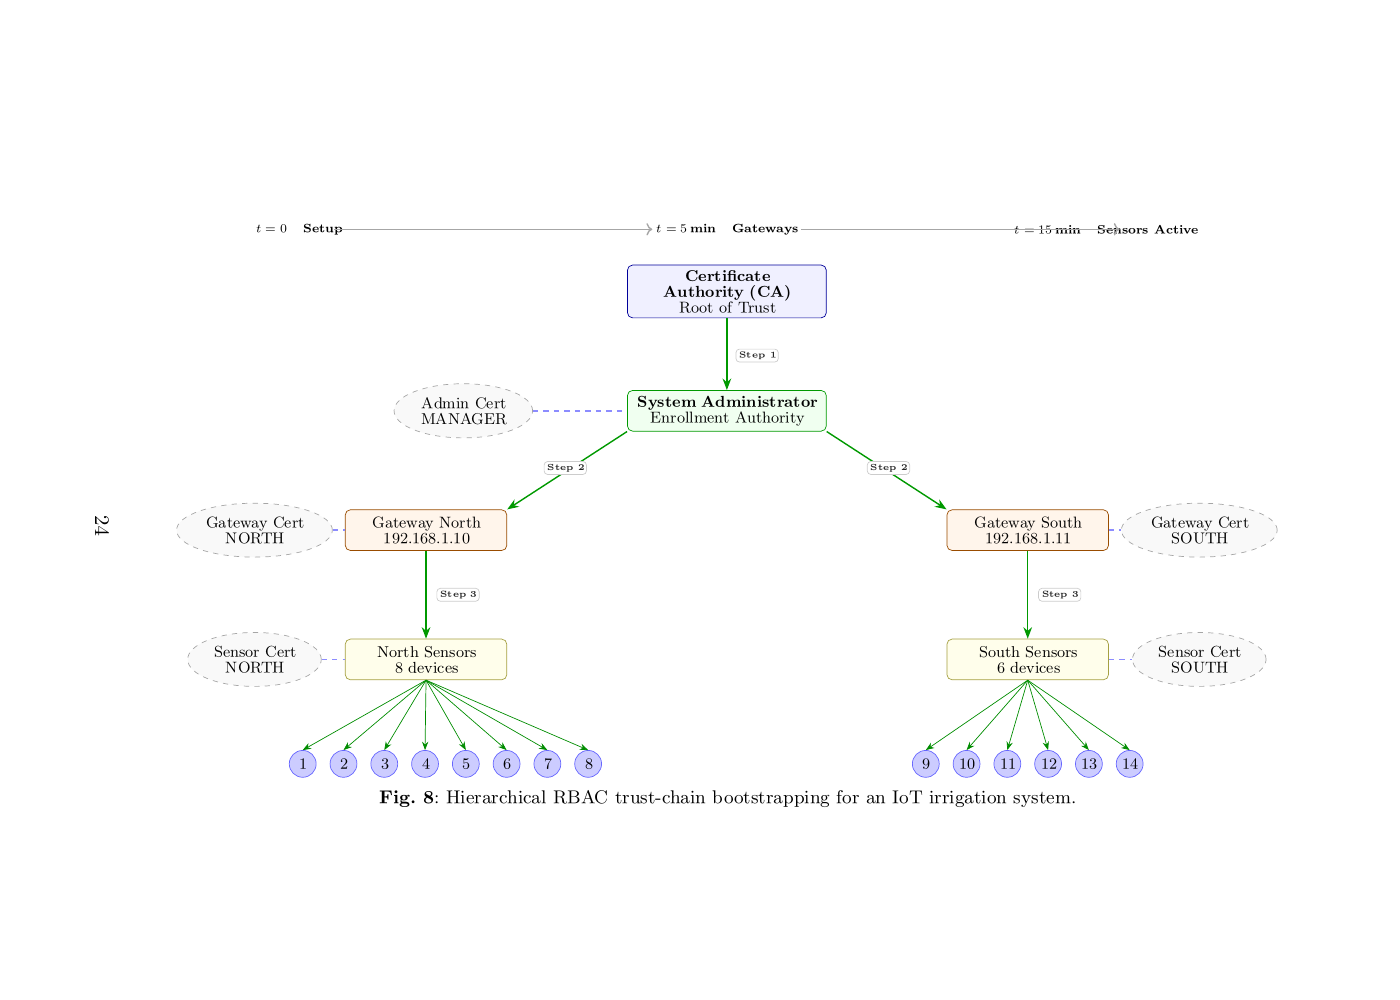
\includegraphics[width=0.85\textwidth]{figures/extracted/beloasone2025-hrbac-trust-chain.png}
  \caption{Hierarchical enrolment chain for the seven-role \gls{hrbac}
           model of Equations~\ref{eq:hrbac_eff}
           and~\ref{eq:hrbac_grant}.}
  \label{fig:hrbac-trust-chain}
\end{figure}

Table~\ref{tab:app-hrbac-matrix} reproduces the permission assignment
$pa(r)$ for every role and resource Chapter Three's chaincode governs, so
that the effective-permission union in Equation~\ref{eq:hrbac_eff} can be
checked against a concrete instance.

\begin{table}[htbp]
\centering
\caption{Permission matrix for agricultural resources across the seven
         \gls{hrbac} roles. \emph{own} = own zone only, \emph{zone} =
         assigned zone, \emph{all} = all zones, N/A = no access.}
\label{tab:app-hrbac-matrix}
\footnotesize
\begin{tabularx}{\textwidth}{@{}p{0.19\textwidth}X X X X X X X@{}}
\toprule
\textbf{Resource} & \textbf{Sensor} & \textbf{Gateway} & \textbf{Farmer} &
  \textbf{Agron.} & \textbf{Cert.} & \textbf{Supply} & \textbf{Admin} \\
\midrule
Sensor data        & own & zone & all  & all & all  & N/A   & all \\
Irrigation control  & N/A & zone & full & N/A & N/A  & N/A   & full \\
Audit logs          & N/A & N/A  & N/A  & N/A & read & N/A   & full \\
Role assignments    & N/A & N/A  & N/A  & N/A & N/A  & N/A   & full \\
Cross-zone tokens   & N/A & N/A  & N/A  & N/A & N/A  & N/A   & issue \\
\bottomrule
\end{tabularx}
{\footnotesize \textit{Note:} Agron. = Agronomist, Cert. = Certification
 Body, Supply = Supply Chain Partner.}
\end{table}

Two rows are worth reading against Equation~\ref{eq:hrbac_grant} directly.
\textbf{Sensor data} is the only resource every role can reach in some
capacity, own-zone write for the sensor itself, zone-scoped read for the
gateway, and unrestricted read for the roles that sit above \textsc{Farmer}
in the partial order above; this is what makes the zone predicate
$\mathrm{zone}(u) = \mathrm{zone}(res)$ load-bearing rather than redundant;
without it, every role above Gateway would read every zone's sensor data
by default. \textbf{Role assignments} and \textbf{cross-zone tokens} are
reachable only by \textsc{Admin}, which is what closes
Equation~\ref{eq:hrbac_grant}'s $\mathrm{czt}(u,\mathrm{zone}(res),t)$
predicate: a cross-zone token can only be minted by the one role whose own
access is already unrestricted, so the token mechanism widens a
requester's reach without ever widening the set of principals who can
create that widening.
) resets the
% chapter counter and switches \thechapter to A, B, C ...; the heading macro
% is redefined alongside it (see main.tex) so headings read "APPENDIX A",
% "APPENDIX B", not a spelled-out number.
%
% Each appendix supplies material referenced but not derived in full in the
% main text, per guide back-matter order: Bibliography, Appendices, Author's
% index, Subject index, CV (PhD only).
% =============================================================================

\chapter{Worked Reconstruction Example for the Chinese Remainder Theorem}
\label{app:crt_worked}

Section~\ref{subsec:lit_crt} states Garner's reconstruction identity
(Equation~\ref{eq:crt_reconstruction}) in general form. This appendix
carries one complete numeric instance through every step, including the
modular-inverse computations that Chapter Two states as results, so that
the arithmetic underlying Chapter Three's implementation is checkable by
hand.

Take the moduli set $\{97, 101, 103\}$, pairwise coprime, with product
\begin{equation*}
M = 97 \times 101 \times 103 = 1{,}009{,}091.
\end{equation*}
A sensor reading of \SI{25.30}{\celsius}, scaled by 100 to keep the value
integral, gives $x = 2530$. Its three residues are
\begin{align*}
r_1 &= 2530 \bmod 97 = 8, \\
r_2 &= 2530 \bmod 101 = 5, \\
r_3 &= 2530 \bmod 103 = 58.
\end{align*}

\paragraph{Step 1: partial products.} For each modulus $m_i$,
$M_i = M / m_i$:
\begin{align*}
M_1 &= 101 \times 103 = 10{,}403, \\
M_2 &= 97 \times 103 = 9{,}991, \\
M_3 &= 97 \times 101 = 9{,}797.
\end{align*}

\paragraph{Step 2: modular inverses.} Each $N_i$ satisfies
$M_i N_i \equiv 1 \pmod{m_i}$. Reducing $M_i$ modulo $m_i$ first keeps the
inverse search small. For $m_1 = 97$:
\begin{align*}
M_1 \bmod 97 &= 10{,}403 \bmod 97 = 24, \\
24 \times 93 &= 2{,}232 = 23 \times 97 + 1
  \;\Rightarrow\; N_1 = 93.
\end{align*}
For $m_2 = 101$:
\begin{align*}
M_2 \bmod 101 &= 9{,}991 \bmod 101 = 93, \\
93 \times 63 &= 5{,}859 = 58 \times 101 + 1
  \;\Rightarrow\; N_2 = 63.
\end{align*}
For $m_3 = 103$:
\begin{align*}
M_3 \bmod 103 &= 9{,}797 \bmod 103 = 12, \\
12 \times 43 &= 516 = 5 \times 103 + 1
  \;\Rightarrow\; N_3 = 43.
\end{align*}
Each inverse is found by inspection here because the moduli are small; the
gateway firmware computes the same quantity with the extended Euclidean
algorithm, $O(\log m_i)$ per modulus, a sub-millisecond cost at this
moduli size (Chapter Three reports measured decomposition and
reconstruction timings).

\paragraph{Step 3: reconstruction.} Substituting into
Equation~\ref{eq:crt_reconstruction}:
\begin{align*}
x &= \bigl( r_1 M_1 N_1 + r_2 M_2 N_2 + r_3 M_3 N_3 \bigr) \bmod M \\
  &= \bigl( 8 \times 10{,}403 \times 93 + 5 \times 9{,}991 \times 63
           + 58 \times 9{,}797 \times 43 \bigr) \bmod 1{,}009{,}091 \\
  &= 2{,}530,
\end{align*}
exact, with zero reconstruction error, recovering \SI{25.30}{\celsius}
after descaling. Losing any one residue, say $r_3$, leaves a unique
solution modulo $m_1 m_2 = 9{,}797$, which happens to be exact for
\emph{this particular} value because $2{,}530 < 9{,}797$.

\paragraph{Why that qualifier matters.} It does not generalise to every
encoded value the firmware produces. The single-sensor value worked above
fits comfortably under any two-modulus product, but the deployed encoding
in \texttt{esp32/main/main.c} packs a soil-moisture reading and a
temperature bucket into one integer, $x = \mathrm{soil}\times 201 +
\mathrm{temp\_bucket}$, precisely so that the full three-modulus budget of
Section~\ref{subsec:lit_crt} is used; with soil scaled to
$[0,4095]$, $x$ reaches up to $823{,}295$, which requires all three
moduli, since no pair's product exceeds $10{,}403$. The gateway's
\texttt{decode} routine (\texttt{gateway/crt\_decode.py}) accepts any two
residues and returns the smallest non-negative solution modulo their
product, documenting that this "matches gateway reassembly for sensor
values constrained below the product of the received moduli" rather than
guaranteeing correctness in general; for a combined value at or above
that product, two-residue decoding returns a different, aliased value
rather than signalling failure. This is why the subset-recovery figure
the source article reports is a measured $64.1\%$ against a $66.7\%$
theoretical figure for two-of-three recovery, not the $100\%$ that would
hold if every encoded value stayed under every two-modulus product; when
Chapter Three's own data-recovery table is written, it should carry the
same measured figure rather than a general bound. The
subset-recovery property of Section~\ref{subsec:lit_crt} is real and
exact for values small enough relative to the moduli in play; it is not,
as deployed here, a blanket guarantee, and Chapter Three's treatment of
loss resilience should state the recovery rate as measured rather than
imply the general bound applies unconditionally.

\chapter{Hierarchical Role-Based Access Control Formalisation and Permission
Matrix}
\label{app:hrbac_matrix}

Chapter Two's review of the access-control literature
(Section~\ref{subsec:lit_privacy}) finds \gls{rbac} enforced in chaincode a
well-established mechanism, generally terminating at the gateway, but no
published, deployed formalisation of a \emph{hierarchical} role structure
with zone and temporal constraints folded into the grant decision itself.
This appendix states the formalisation we develop to close that gap and
that Chapter Three's chaincode implements, so that it is available for
reference wherever the main chapters invoke it, without presenting our own
model as part of the literature under review.

We extend flat \gls{rbac} with a role hierarchy expressed as a partial
order $\preceq$ over the role set $R$, where $r_i \preceq r_j$ iff
$\mathrm{permissions}(r_i) \subseteq \mathrm{permissions}(r_j)$, so that a
user $u$'s effective permission set in a session is the union across every
role dominated by an active role,
\begin{equation}
\mathrm{eff}(u) = \bigcup_{r \in \mathrm{active}(u)} \; \bigcup_{r' \preceq r} pa(r'),
\label{eq:hrbac_eff}
\end{equation}
with $pa(r)$ the permissions directly assigned to role $r$. An access
request $(u, op, res, t)$ is then granted only if an active, non-expired
role of $u$ carries the requested permission \emph{and} the requester's
zone matches the resource's zone or the requester holds an
administrator-issued cross-zone token,
\begin{equation}
\exists\, r \in \mathrm{active}(u,t) : (op,res) \in \mathrm{eff}(r)
\;\land\; \bigl(\mathrm{zone}(u) = \mathrm{zone}(res) \lor
\mathrm{czt}(u,\mathrm{zone}(res),t)\bigr),
\label{eq:hrbac_grant}
\end{equation}
which folds zone and temporal constraints directly into the access
decision rather than leaving them to an external policy layer. This
follows the general tradition of administrative role hierarchies in
access-control theory~\cite{lu2022revocation} and shares its enforcement
point, the chaincode's client-identity check, with the wider Fabric
access-control literature~\cite{mdpiAccessControl}, but authenticates at
the individual sensing node rather than only at the gateway holding the
\gls{x509} certificate that signs the transaction.
Figure~\ref{fig:hrbac-trust-chain} shows the resulting enrolment chain,
root certificate authority down through gateways to individual sensing
nodes.

\begin{figure}[htbp]
  \centering
  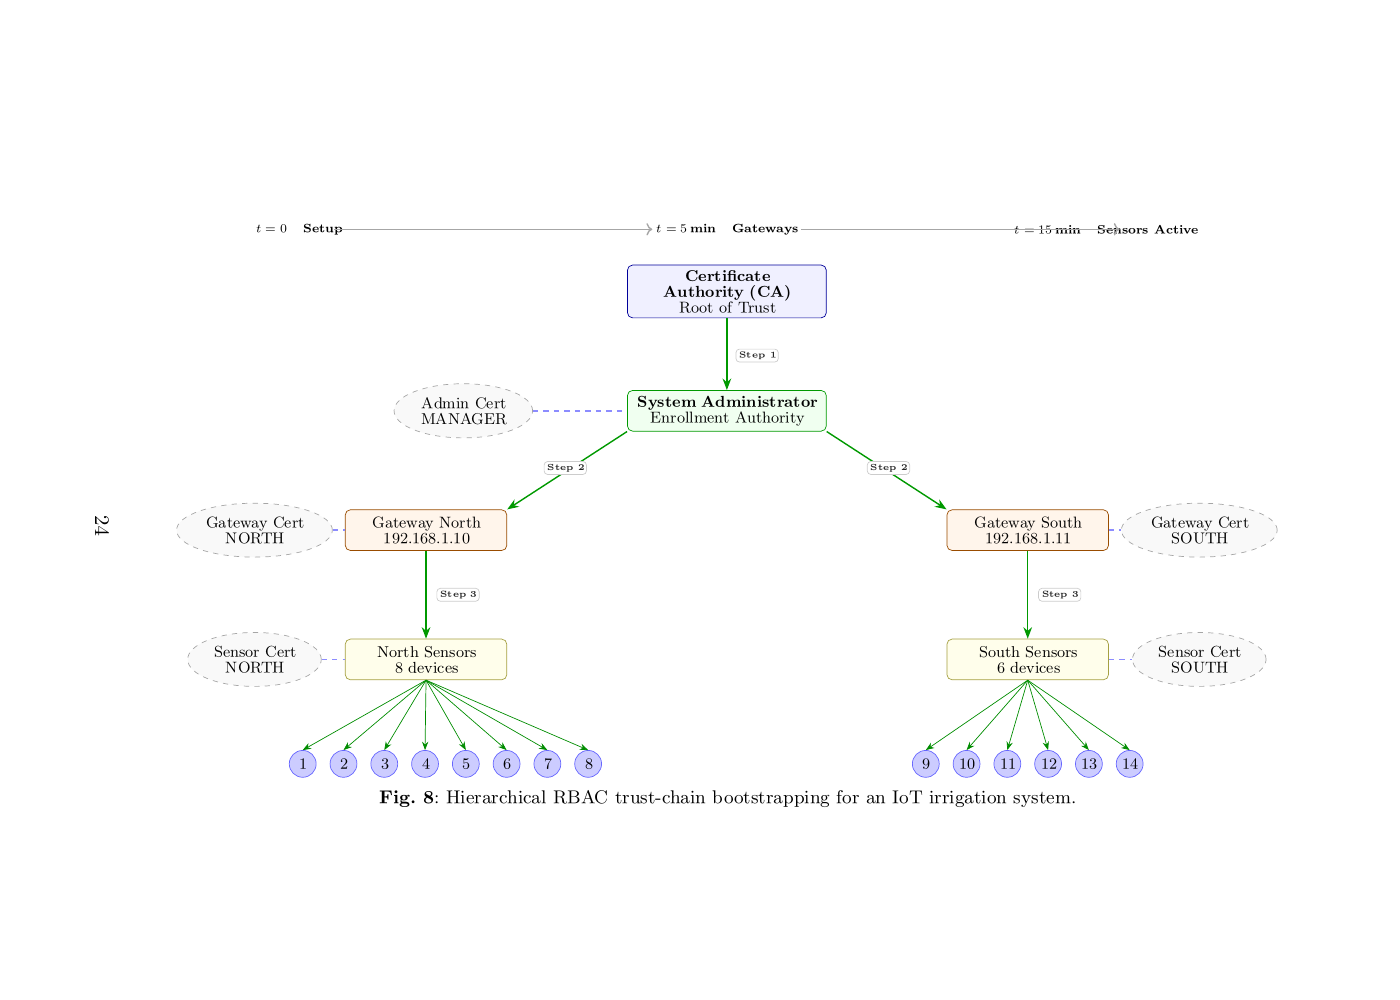
\includegraphics[width=0.85\textwidth]{figures/extracted/beloasone2025-hrbac-trust-chain.png}
  \caption{Hierarchical enrolment chain for the seven-role \gls{hrbac}
           model of Equations~\ref{eq:hrbac_eff}
           and~\ref{eq:hrbac_grant}.}
  \label{fig:hrbac-trust-chain}
\end{figure}

Table~\ref{tab:app-hrbac-matrix} reproduces the permission assignment
$pa(r)$ for every role and resource Chapter Three's chaincode governs, so
that the effective-permission union in Equation~\ref{eq:hrbac_eff} can be
checked against a concrete instance.

\begin{table}[htbp]
\centering
\caption{Permission matrix for agricultural resources across the seven
         \gls{hrbac} roles. \emph{own} = own zone only, \emph{zone} =
         assigned zone, \emph{all} = all zones, N/A = no access.}
\label{tab:app-hrbac-matrix}
\footnotesize
\begin{tabularx}{\textwidth}{@{}p{0.19\textwidth}X X X X X X X@{}}
\toprule
\textbf{Resource} & \textbf{Sensor} & \textbf{Gateway} & \textbf{Farmer} &
  \textbf{Agron.} & \textbf{Cert.} & \textbf{Supply} & \textbf{Admin} \\
\midrule
Sensor data        & own & zone & all  & all & all  & N/A   & all \\
Irrigation control  & N/A & zone & full & N/A & N/A  & N/A   & full \\
Audit logs          & N/A & N/A  & N/A  & N/A & read & N/A   & full \\
Role assignments    & N/A & N/A  & N/A  & N/A & N/A  & N/A   & full \\
Cross-zone tokens   & N/A & N/A  & N/A  & N/A & N/A  & N/A   & issue \\
\bottomrule
\end{tabularx}
{\footnotesize \textit{Note:} Agron. = Agronomist, Cert. = Certification
 Body, Supply = Supply Chain Partner.}
\end{table}

Two rows are worth reading against Equation~\ref{eq:hrbac_grant} directly.
\textbf{Sensor data} is the only resource every role can reach in some
capacity, own-zone write for the sensor itself, zone-scoped read for the
gateway, and unrestricted read for the roles that sit above \textsc{Farmer}
in the partial order above; this is what makes the zone predicate
$\mathrm{zone}(u) = \mathrm{zone}(res)$ load-bearing rather than redundant;
without it, every role above Gateway would read every zone's sensor data
by default. \textbf{Role assignments} and \textbf{cross-zone tokens} are
reachable only by \textsc{Admin}, which is what closes
Equation~\ref{eq:hrbac_grant}'s $\mathrm{czt}(u,\mathrm{zone}(res),t)$
predicate: a cross-zone token can only be minted by the one role whose own
access is already unrestricted, so the token mechanism widens a
requester's reach without ever widening the set of principals who can
create that widening.
) resets the
% chapter counter and switches \thechapter to A, B, C ...; the heading macro
% is redefined alongside it (see main.tex) so headings read "APPENDIX A",
% "APPENDIX B", not a spelled-out number.
%
% Each appendix supplies material referenced but not derived in full in the
% main text, per guide back-matter order: Bibliography, Appendices, Author's
% index, Subject index, CV (PhD only).
% =============================================================================

\chapter{Worked Reconstruction Example for the Chinese Remainder Theorem}
\label{app:crt_worked}

Section~\ref{subsec:lit_crt} states Garner's reconstruction identity
(Equation~\ref{eq:crt_reconstruction}) in general form. This appendix
carries one complete numeric instance through every step, including the
modular-inverse computations that Chapter Two states as results, so that
the arithmetic underlying Chapter Three's implementation is checkable by
hand.

Take the moduli set $\{97, 101, 103\}$, pairwise coprime, with product
\begin{equation*}
M = 97 \times 101 \times 103 = 1{,}009{,}091.
\end{equation*}
A sensor reading of \SI{25.30}{\celsius}, scaled by 100 to keep the value
integral, gives $x = 2530$. Its three residues are
\begin{align*}
r_1 &= 2530 \bmod 97 = 8, \\
r_2 &= 2530 \bmod 101 = 5, \\
r_3 &= 2530 \bmod 103 = 58.
\end{align*}

\paragraph{Step 1: partial products.} For each modulus $m_i$,
$M_i = M / m_i$:
\begin{align*}
M_1 &= 101 \times 103 = 10{,}403, \\
M_2 &= 97 \times 103 = 9{,}991, \\
M_3 &= 97 \times 101 = 9{,}797.
\end{align*}

\paragraph{Step 2: modular inverses.} Each $N_i$ satisfies
$M_i N_i \equiv 1 \pmod{m_i}$. Reducing $M_i$ modulo $m_i$ first keeps the
inverse search small. For $m_1 = 97$:
\begin{align*}
M_1 \bmod 97 &= 10{,}403 \bmod 97 = 24, \\
24 \times 93 &= 2{,}232 = 23 \times 97 + 1
  \;\Rightarrow\; N_1 = 93.
\end{align*}
For $m_2 = 101$:
\begin{align*}
M_2 \bmod 101 &= 9{,}991 \bmod 101 = 93, \\
93 \times 63 &= 5{,}859 = 58 \times 101 + 1
  \;\Rightarrow\; N_2 = 63.
\end{align*}
For $m_3 = 103$:
\begin{align*}
M_3 \bmod 103 &= 9{,}797 \bmod 103 = 12, \\
12 \times 43 &= 516 = 5 \times 103 + 1
  \;\Rightarrow\; N_3 = 43.
\end{align*}
Each inverse is found by inspection here because the moduli are small; the
gateway firmware computes the same quantity with the extended Euclidean
algorithm, $O(\log m_i)$ per modulus, a sub-millisecond cost at this
moduli size (Chapter Three reports measured decomposition and
reconstruction timings).

\paragraph{Step 3: reconstruction.} Substituting into
Equation~\ref{eq:crt_reconstruction}:
\begin{align*}
x &= \bigl( r_1 M_1 N_1 + r_2 M_2 N_2 + r_3 M_3 N_3 \bigr) \bmod M \\
  &= \bigl( 8 \times 10{,}403 \times 93 + 5 \times 9{,}991 \times 63
           + 58 \times 9{,}797 \times 43 \bigr) \bmod 1{,}009{,}091 \\
  &= 2{,}530,
\end{align*}
exact, with zero reconstruction error, recovering \SI{25.30}{\celsius}
after descaling. Losing any one residue, say $r_3$, leaves a unique
solution modulo $m_1 m_2 = 9{,}797$, which happens to be exact for
\emph{this particular} value because $2{,}530 < 9{,}797$.

\paragraph{Why that qualifier matters.} It does not generalise to every
encoded value the firmware produces. The single-sensor value worked above
fits comfortably under any two-modulus product, but the deployed encoding
in \texttt{esp32/main/main.c} packs a soil-moisture reading and a
temperature bucket into one integer, $x = \mathrm{soil}\times 201 +
\mathrm{temp\_bucket}$, precisely so that the full three-modulus budget of
Section~\ref{subsec:lit_crt} is used; with soil scaled to
$[0,4095]$, $x$ reaches up to $823{,}295$, which requires all three
moduli, since no pair's product exceeds $10{,}403$. The gateway's
\texttt{decode} routine (\texttt{gateway/crt\_decode.py}) accepts any two
residues and returns the smallest non-negative solution modulo their
product, documenting that this "matches gateway reassembly for sensor
values constrained below the product of the received moduli" rather than
guaranteeing correctness in general; for a combined value at or above
that product, two-residue decoding returns a different, aliased value
rather than signalling failure. This is why the subset-recovery figure
the source article reports is a measured $64.1\%$ against a $66.7\%$
theoretical figure for two-of-three recovery, not the $100\%$ that would
hold if every encoded value stayed under every two-modulus product; when
Chapter Three's own data-recovery table is written, it should carry the
same measured figure rather than a general bound. The
subset-recovery property of Section~\ref{subsec:lit_crt} is real and
exact for values small enough relative to the moduli in play; it is not,
as deployed here, a blanket guarantee, and Chapter Three's treatment of
loss resilience should state the recovery rate as measured rather than
imply the general bound applies unconditionally.

\chapter{Hierarchical Role-Based Access Control Formalisation and Permission
Matrix}
\label{app:hrbac_matrix}

Chapter Two's review of the access-control literature
(Section~\ref{subsec:lit_privacy}) finds \gls{rbac} enforced in chaincode a
well-established mechanism, generally terminating at the gateway, but no
published, deployed formalisation of a \emph{hierarchical} role structure
with zone and temporal constraints folded into the grant decision itself.
This appendix states the formalisation we develop to close that gap and
that Chapter Three's chaincode implements, so that it is available for
reference wherever the main chapters invoke it, without presenting our own
model as part of the literature under review.

We extend flat \gls{rbac} with a role hierarchy expressed as a partial
order $\preceq$ over the role set $R$, where $r_i \preceq r_j$ iff
$\mathrm{permissions}(r_i) \subseteq \mathrm{permissions}(r_j)$, so that a
user $u$'s effective permission set in a session is the union across every
role dominated by an active role,
\begin{equation}
\mathrm{eff}(u) = \bigcup_{r \in \mathrm{active}(u)} \; \bigcup_{r' \preceq r} pa(r'),
\label{eq:hrbac_eff}
\end{equation}
with $pa(r)$ the permissions directly assigned to role $r$. An access
request $(u, op, res, t)$ is then granted only if an active, non-expired
role of $u$ carries the requested permission \emph{and} the requester's
zone matches the resource's zone or the requester holds an
administrator-issued cross-zone token,
\begin{equation}
\exists\, r \in \mathrm{active}(u,t) : (op,res) \in \mathrm{eff}(r)
\;\land\; \bigl(\mathrm{zone}(u) = \mathrm{zone}(res) \lor
\mathrm{czt}(u,\mathrm{zone}(res),t)\bigr),
\label{eq:hrbac_grant}
\end{equation}
which folds zone and temporal constraints directly into the access
decision rather than leaving them to an external policy layer. This
follows the general tradition of administrative role hierarchies in
access-control theory~\cite{lu2022revocation} and shares its enforcement
point, the chaincode's client-identity check, with the wider Fabric
access-control literature~\cite{mdpiAccessControl}, but authenticates at
the individual sensing node rather than only at the gateway holding the
\gls{x509} certificate that signs the transaction.
Figure~\ref{fig:hrbac-trust-chain} shows the resulting enrolment chain,
root certificate authority down through gateways to individual sensing
nodes.

\begin{figure}[htbp]
  \centering
  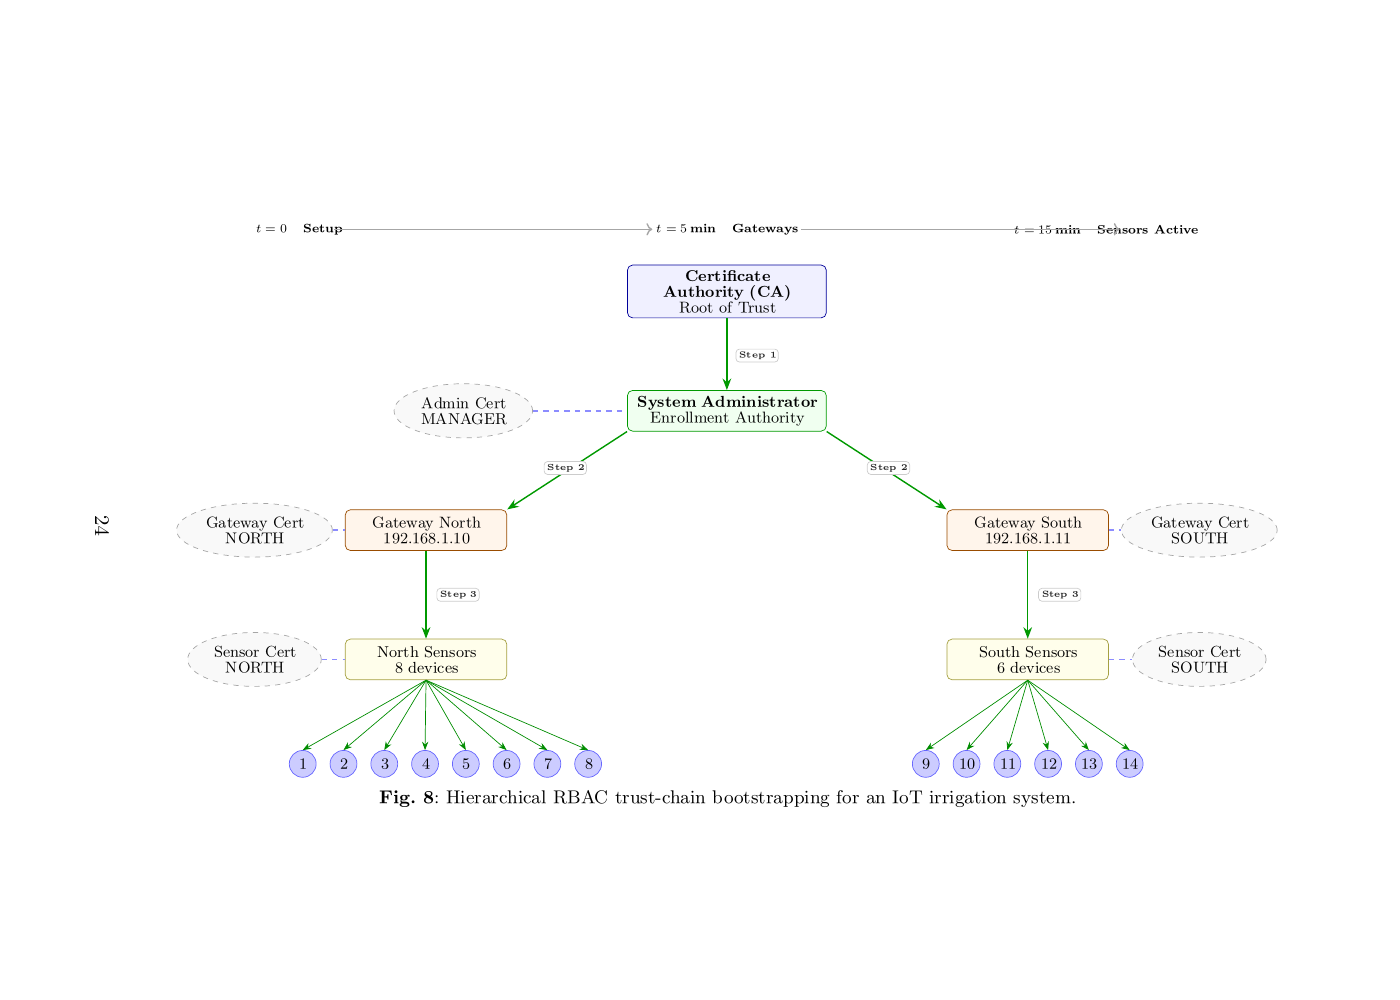
\includegraphics[width=0.85\textwidth]{figures/extracted/beloasone2025-hrbac-trust-chain.png}
  \caption{Hierarchical enrolment chain for the seven-role \gls{hrbac}
           model of Equations~\ref{eq:hrbac_eff}
           and~\ref{eq:hrbac_grant}.}
  \label{fig:hrbac-trust-chain}
\end{figure}

Table~\ref{tab:app-hrbac-matrix} reproduces the permission assignment
$pa(r)$ for every role and resource Chapter Three's chaincode governs, so
that the effective-permission union in Equation~\ref{eq:hrbac_eff} can be
checked against a concrete instance.

\begin{table}[htbp]
\centering
\caption{Permission matrix for agricultural resources across the seven
         \gls{hrbac} roles. \emph{own} = own zone only, \emph{zone} =
         assigned zone, \emph{all} = all zones, N/A = no access.}
\label{tab:app-hrbac-matrix}
\footnotesize
\begin{tabularx}{\textwidth}{@{}p{0.19\textwidth}X X X X X X X@{}}
\toprule
\textbf{Resource} & \textbf{Sensor} & \textbf{Gateway} & \textbf{Farmer} &
  \textbf{Agron.} & \textbf{Cert.} & \textbf{Supply} & \textbf{Admin} \\
\midrule
Sensor data        & own & zone & all  & all & all  & N/A   & all \\
Irrigation control  & N/A & zone & full & N/A & N/A  & N/A   & full \\
Audit logs          & N/A & N/A  & N/A  & N/A & read & N/A   & full \\
Role assignments    & N/A & N/A  & N/A  & N/A & N/A  & N/A   & full \\
Cross-zone tokens   & N/A & N/A  & N/A  & N/A & N/A  & N/A   & issue \\
\bottomrule
\end{tabularx}
{\footnotesize \textit{Note:} Agron. = Agronomist, Cert. = Certification
 Body, Supply = Supply Chain Partner.}
\end{table}

Two rows are worth reading against Equation~\ref{eq:hrbac_grant} directly.
\textbf{Sensor data} is the only resource every role can reach in some
capacity, own-zone write for the sensor itself, zone-scoped read for the
gateway, and unrestricted read for the roles that sit above \textsc{Farmer}
in the partial order above; this is what makes the zone predicate
$\mathrm{zone}(u) = \mathrm{zone}(res)$ load-bearing rather than redundant;
without it, every role above Gateway would read every zone's sensor data
by default. \textbf{Role assignments} and \textbf{cross-zone tokens} are
reachable only by \textsc{Admin}, which is what closes
Equation~\ref{eq:hrbac_grant}'s $\mathrm{czt}(u,\mathrm{zone}(res),t)$
predicate: a cross-zone token can only be minted by the one role whose own
access is already unrestricted, so the token mechanism widens a
requester's reach without ever widening the set of principals who can
create that widening.
) resets the
% chapter counter and switches \thechapter to A, B, C ...; the heading macro
% is redefined alongside it (see main.tex) so headings read "APPENDIX A",
% "APPENDIX B", not a spelled-out number.
%
% Each appendix supplies material referenced but not derived in full in the
% main text, per guide back-matter order: Bibliography, Appendices, Author's
% index, Subject index, CV (PhD only).
% =============================================================================

\chapter{Worked Reconstruction Example for the Chinese Remainder Theorem}
\label{app:crt_worked}

Section~\ref{subsec:lit_crt} states Garner's reconstruction identity
(Equation~\ref{eq:crt_reconstruction}) in general form. This appendix
carries one complete numeric instance through every step, including the
modular-inverse computations that Chapter Two states as results, so that
the arithmetic underlying Chapter Three's implementation is checkable by
hand.

Take the moduli set $\{97, 101, 103\}$, pairwise coprime, with product
\begin{equation*}
M = 97 \times 101 \times 103 = 1{,}009{,}091.
\end{equation*}
A sensor reading of \SI{25.30}{\celsius}, scaled by 100 to keep the value
integral, gives $x = 2530$. Its three residues are
\begin{align*}
r_1 &= 2530 \bmod 97 = 8, \\
r_2 &= 2530 \bmod 101 = 5, \\
r_3 &= 2530 \bmod 103 = 58.
\end{align*}

\paragraph{Step 1: partial products.} For each modulus $m_i$,
$M_i = M / m_i$:
\begin{align*}
M_1 &= 101 \times 103 = 10{,}403, \\
M_2 &= 97 \times 103 = 9{,}991, \\
M_3 &= 97 \times 101 = 9{,}797.
\end{align*}

\paragraph{Step 2: modular inverses.} Each $N_i$ satisfies
$M_i N_i \equiv 1 \pmod{m_i}$. Reducing $M_i$ modulo $m_i$ first keeps the
inverse search small. For $m_1 = 97$:
\begin{align*}
M_1 \bmod 97 &= 10{,}403 \bmod 97 = 24, \\
24 \times 93 &= 2{,}232 = 23 \times 97 + 1
  \;\Rightarrow\; N_1 = 93.
\end{align*}
For $m_2 = 101$:
\begin{align*}
M_2 \bmod 101 &= 9{,}991 \bmod 101 = 93, \\
93 \times 63 &= 5{,}859 = 58 \times 101 + 1
  \;\Rightarrow\; N_2 = 63.
\end{align*}
For $m_3 = 103$:
\begin{align*}
M_3 \bmod 103 &= 9{,}797 \bmod 103 = 12, \\
12 \times 43 &= 516 = 5 \times 103 + 1
  \;\Rightarrow\; N_3 = 43.
\end{align*}
Each inverse is found by inspection here because the moduli are small; the
gateway firmware computes the same quantity with the extended Euclidean
algorithm, $O(\log m_i)$ per modulus, a sub-millisecond cost at this
moduli size (Chapter Three reports measured decomposition and
reconstruction timings).

\paragraph{Step 3: reconstruction.} Substituting into
Equation~\ref{eq:crt_reconstruction}:
\begin{align*}
x &= \bigl( r_1 M_1 N_1 + r_2 M_2 N_2 + r_3 M_3 N_3 \bigr) \bmod M \\
  &= \bigl( 8 \times 10{,}403 \times 93 + 5 \times 9{,}991 \times 63
           + 58 \times 9{,}797 \times 43 \bigr) \bmod 1{,}009{,}091 \\
  &= 2{,}530,
\end{align*}
exact, with zero reconstruction error, recovering \SI{25.30}{\celsius}
after descaling. Losing any one residue, say $r_3$, leaves a unique
solution modulo $m_1 m_2 = 9{,}797$, which happens to be exact for
\emph{this particular} value because $2{,}530 < 9{,}797$.

\paragraph{Why that qualifier matters.} It does not generalise to every
encoded value the firmware produces. The single-sensor value worked above
fits comfortably under any two-modulus product, but the deployed encoding
in \texttt{esp32/main/main.c} packs a soil-moisture reading and a
temperature bucket into one integer, $x = \mathrm{soil}\times 201 +
\mathrm{temp\_bucket}$, precisely so that the full three-modulus budget of
Section~\ref{subsec:lit_crt} is used; with soil scaled to
$[0,4095]$, $x$ reaches up to $823{,}295$, which requires all three
moduli, since no pair's product exceeds $10{,}403$. The gateway's
\texttt{decode} routine (\texttt{gateway/crt\_decode.py}) accepts any two
residues and returns the smallest non-negative solution modulo their
product, documenting that this "matches gateway reassembly for sensor
values constrained below the product of the received moduli" rather than
guaranteeing correctness in general; for a combined value at or above
that product, two-residue decoding returns a different, aliased value
rather than signalling failure. This is why the subset-recovery figure
the source article reports is a measured $64.1\%$ against a $66.7\%$
theoretical figure for two-of-three recovery, not the $100\%$ that would
hold if every encoded value stayed under every two-modulus product; when
Chapter Three's own data-recovery table is written, it should carry the
same measured figure rather than a general bound. The
subset-recovery property of Section~\ref{subsec:lit_crt} is real and
exact for values small enough relative to the moduli in play; it is not,
as deployed here, a blanket guarantee, and Chapter Three's treatment of
loss resilience should state the recovery rate as measured rather than
imply the general bound applies unconditionally.

\chapter{Hierarchical Role-Based Access Control Formalisation and Permission
Matrix}
\label{app:hrbac_matrix}

Chapter Two's review of the access-control literature
(Section~\ref{subsec:lit_privacy}) finds \gls{rbac} enforced in chaincode a
well-established mechanism, generally terminating at the gateway, but no
published, deployed formalisation of a \emph{hierarchical} role structure
with zone and temporal constraints folded into the grant decision itself.
This appendix states the formalisation we develop to close that gap and
that Chapter Three's chaincode implements, so that it is available for
reference wherever the main chapters invoke it, without presenting our own
model as part of the literature under review.

We extend flat \gls{rbac} with a role hierarchy expressed as a partial
order $\preceq$ over the role set $R$, where $r_i \preceq r_j$ iff
$\mathrm{permissions}(r_i) \subseteq \mathrm{permissions}(r_j)$, so that a
user $u$'s effective permission set in a session is the union across every
role dominated by an active role,
\begin{equation}
\mathrm{eff}(u) = \bigcup_{r \in \mathrm{active}(u)} \; \bigcup_{r' \preceq r} pa(r'),
\label{eq:hrbac_eff}
\end{equation}
with $pa(r)$ the permissions directly assigned to role $r$. An access
request $(u, op, res, t)$ is then granted only if an active, non-expired
role of $u$ carries the requested permission \emph{and} the requester's
zone matches the resource's zone or the requester holds an
administrator-issued cross-zone token,
\begin{equation}
\exists\, r \in \mathrm{active}(u,t) : (op,res) \in \mathrm{eff}(r)
\;\land\; \bigl(\mathrm{zone}(u) = \mathrm{zone}(res) \lor
\mathrm{czt}(u,\mathrm{zone}(res),t)\bigr),
\label{eq:hrbac_grant}
\end{equation}
which folds zone and temporal constraints directly into the access
decision rather than leaving them to an external policy layer. This
follows the general tradition of administrative role hierarchies in
access-control theory~\cite{lu2022revocation} and shares its enforcement
point, the chaincode's client-identity check, with the wider Fabric
access-control literature~\cite{mdpiAccessControl}, but authenticates at
the individual sensing node rather than only at the gateway holding the
\gls{x509} certificate that signs the transaction.
Figure~\ref{fig:hrbac-trust-chain} shows the resulting enrolment chain,
root certificate authority down through gateways to individual sensing
nodes.

\begin{figure}[htbp]
  \centering
  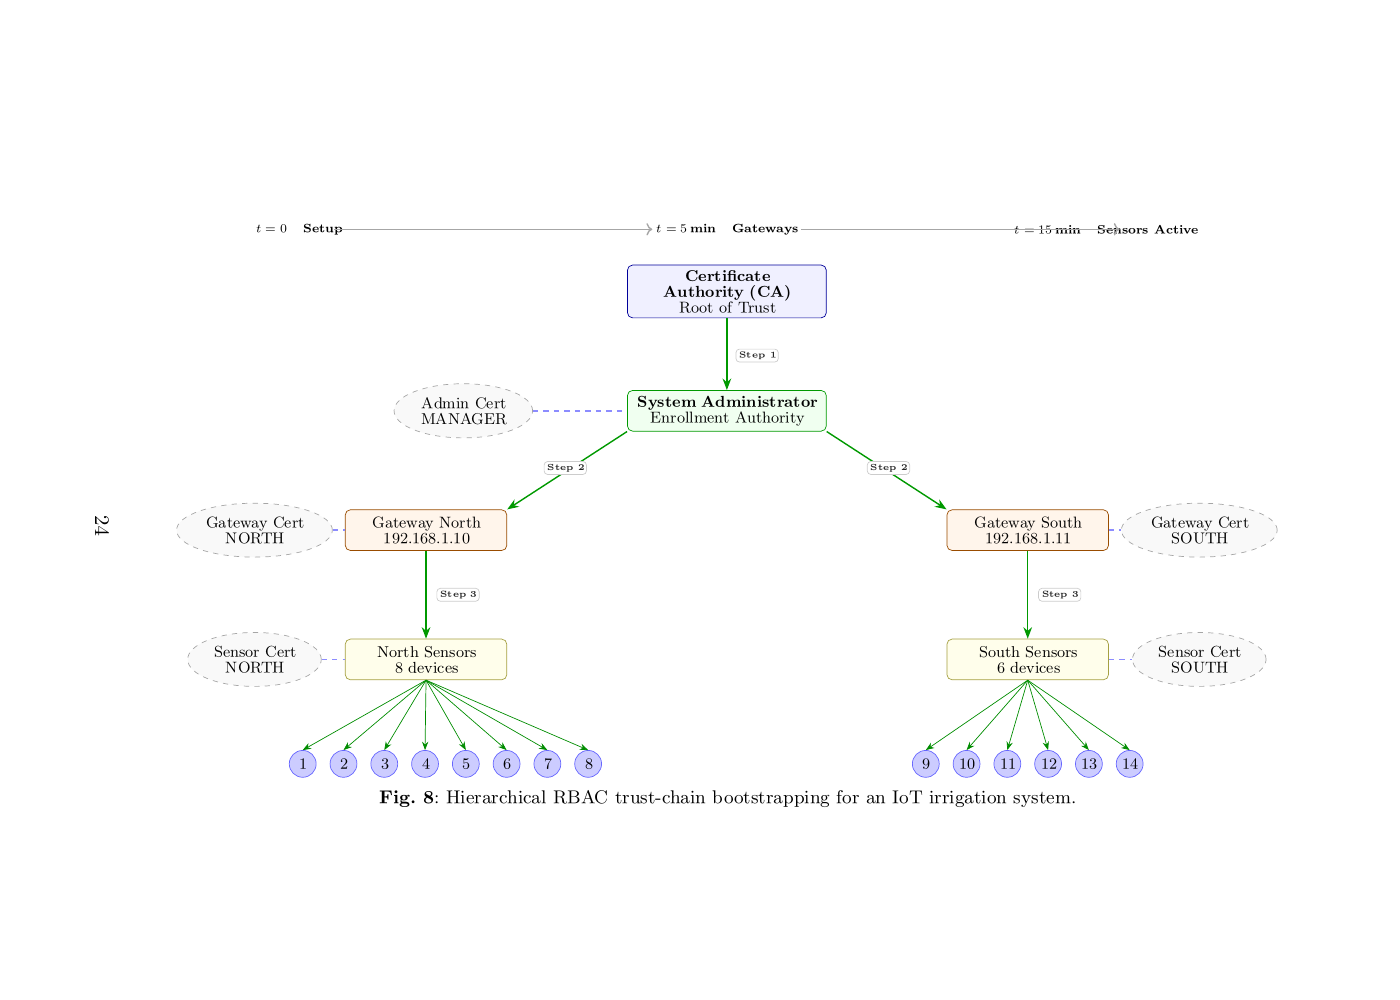
\includegraphics[width=0.85\textwidth]{figures/extracted/beloasone2025-hrbac-trust-chain.png}
  \caption{Hierarchical enrolment chain for the seven-role \gls{hrbac}
           model of Equations~\ref{eq:hrbac_eff}
           and~\ref{eq:hrbac_grant}.}
  \label{fig:hrbac-trust-chain}
\end{figure}

Table~\ref{tab:app-hrbac-matrix} reproduces the permission assignment
$pa(r)$ for every role and resource Chapter Three's chaincode governs, so
that the effective-permission union in Equation~\ref{eq:hrbac_eff} can be
checked against a concrete instance.

\begin{table}[htbp]
\centering
\caption{Permission matrix for agricultural resources across the seven
         \gls{hrbac} roles. \emph{own} = own zone only, \emph{zone} =
         assigned zone, \emph{all} = all zones, N/A = no access.}
\label{tab:app-hrbac-matrix}
\footnotesize
\begin{tabularx}{\textwidth}{@{}p{0.19\textwidth}X X X X X X X@{}}
\toprule
\textbf{Resource} & \textbf{Sensor} & \textbf{Gateway} & \textbf{Farmer} &
  \textbf{Agron.} & \textbf{Cert.} & \textbf{Supply} & \textbf{Admin} \\
\midrule
Sensor data        & own & zone & all  & all & all  & N/A   & all \\
Irrigation control  & N/A & zone & full & N/A & N/A  & N/A   & full \\
Audit logs          & N/A & N/A  & N/A  & N/A & read & N/A   & full \\
Role assignments    & N/A & N/A  & N/A  & N/A & N/A  & N/A   & full \\
Cross-zone tokens   & N/A & N/A  & N/A  & N/A & N/A  & N/A   & issue \\
\bottomrule
\end{tabularx}
{\footnotesize \textit{Note:} Agron. = Agronomist, Cert. = Certification
 Body, Supply = Supply Chain Partner.}
\end{table}

Two rows are worth reading against Equation~\ref{eq:hrbac_grant} directly.
\textbf{Sensor data} is the only resource every role can reach in some
capacity, own-zone write for the sensor itself, zone-scoped read for the
gateway, and unrestricted read for the roles that sit above \textsc{Farmer}
in the partial order above; this is what makes the zone predicate
$\mathrm{zone}(u) = \mathrm{zone}(res)$ load-bearing rather than redundant;
without it, every role above Gateway would read every zone's sensor data
by default. \textbf{Role assignments} and \textbf{cross-zone tokens} are
reachable only by \textsc{Admin}, which is what closes
Equation~\ref{eq:hrbac_grant}'s $\mathrm{czt}(u,\mathrm{zone}(res),t)$
predicate: a cross-zone token can only be minted by the one role whose own
access is already unrestricted, so the token mechanism widens a
requester's reach without ever widening the set of principals who can
create that widening.
